\section{RESULTADOS}

\subsection{Convergência de Malha}

\begin{table}[H]
\centering
\caption{Resultado da análise de convergência de malha.}
\begin{tabular}{|c|c|c|c|c|} 
\hline
Tamanho de Malha & $\lambda_{critico}$ & DOF  & 1ª Frequência (\si{Hz}) & 2ª Frequência (\si{Hz}) \\ \hline
10x10            & \num{524,34}    & \num{606}  & \num{79,80}         & \num{198,50}        \\ \hline
20x20            & \num{518,67}    & \num{2406} & \num{80,48}         & \num{200,92}        \\ \hline
30x30            & \num{517,81}    & \num{5406} & \num{80,64}         & \num{201,49}        \\ \hline
40x40            & \num{517,07}    & \num{9606} & \num{80,69}         & \num{201,70}        \\ \hline
\end{tabular}
\label{tab-result-conv}   
\end{table}

Analisando-se quatro casos com $N$ de 1 até 4 obteve-se os valores
dispostos na tabela \ref{tab-result-conv} de $\lambda$, graus de
liberdade estimados do modelo (DOF), e as duas primeiras frequências
de vibração computadas.


Os erros comparados com a literatura estão dispostos na tabela 
\ref{tab-result-conv-comp}.
Foram utilizados os parâmetros $\beta a/b = \num{2,83}$ e $\mu/M = 
\num{0,0291}$ para a interpolação dos valores das tabelas de
\cite{hedgepeth_flutter_1957} e \cite{pegado_metodo_2003}, 
respectivamente, obtendo-se os valores de $\lambda$ de \num{496,19} e 
\num{515,15}, respectivamente. Os valores teóricos das frequências são
$f_1 = \SI{80.88}{Hz}$ e $f_2 = \SI{202.20}{Hz}$

\begin{table}[H]
\centering
\caption{Resultado comparativo da convergência de malha com a literatura.}
\begin{tabular}{|c|c|c|c|c|}
\hline
\multirow{2}{*}{Tamanho de Malha} & \multicolumn{4}{c|}{Erro Percentual}                 \\ \cline{2-5} 
                                  & Hedgepeth (1957) & Pegado (2003) & $f_1$   & $f_2$   \\ \hline
10x10                             & \SI{5.67}{\percent}           & \SI{1.78}{\percent}         & \SI{-1.34}{\percent}  & \SI{-1.83}{\percent}  \\ \hline
20x20                             & \SI{4.53}{\percent}           & \SI{0.68}{\percent}         & \SI{-0.50}{\percent}  & \SI{-0.64}{\percent}  \\ \hline
30x30                             & \SI{4.36}{\percent}           & \SI{0.52}{\percent}         & \SI{-0.30}{\percent}  & \SI{-0.35}{\percent}  \\ \hline
40x40                             & \SI{4.21}{\percent}           & \SI{0.37}{\percent}         & \SI{-0.24}{\percent}  & \SI{-0.25}{\percent}  \\ \hline
\end{tabular}
\label{tab-result-conv-comp}
\end{table}

\subsection{Placa em Material Composto}

Utilizando-se a malha 20x20 realizou-se a análise obtendo-se os 
valores de $\lambda$ em função de $\theta^*$, comparados com o 
resultado obtido por \cite{sawyer_flutter_1977}, conforme a Figura 
\ref{fig-result-comp}. O parâmetro $\lambda^*$ é semelhante ao 
utilizado anteriormente, entretanto, como a rigidez à flexão da 
placa se torna matricial devido a natureza do material composto, 
utiliza-se $\bar{D}_{11}$ com $\theta = 0$ como valor de referência.
O valor de $\bar{D}_{11}$ pode ser computado facilmente na maioria 
dos \emph{softwares} que suportam análise de laminados.

\begin{figure}[H]
\centering
\caption{Valores de pressão dinâmica adimensional crítica em função da orientação do material.}
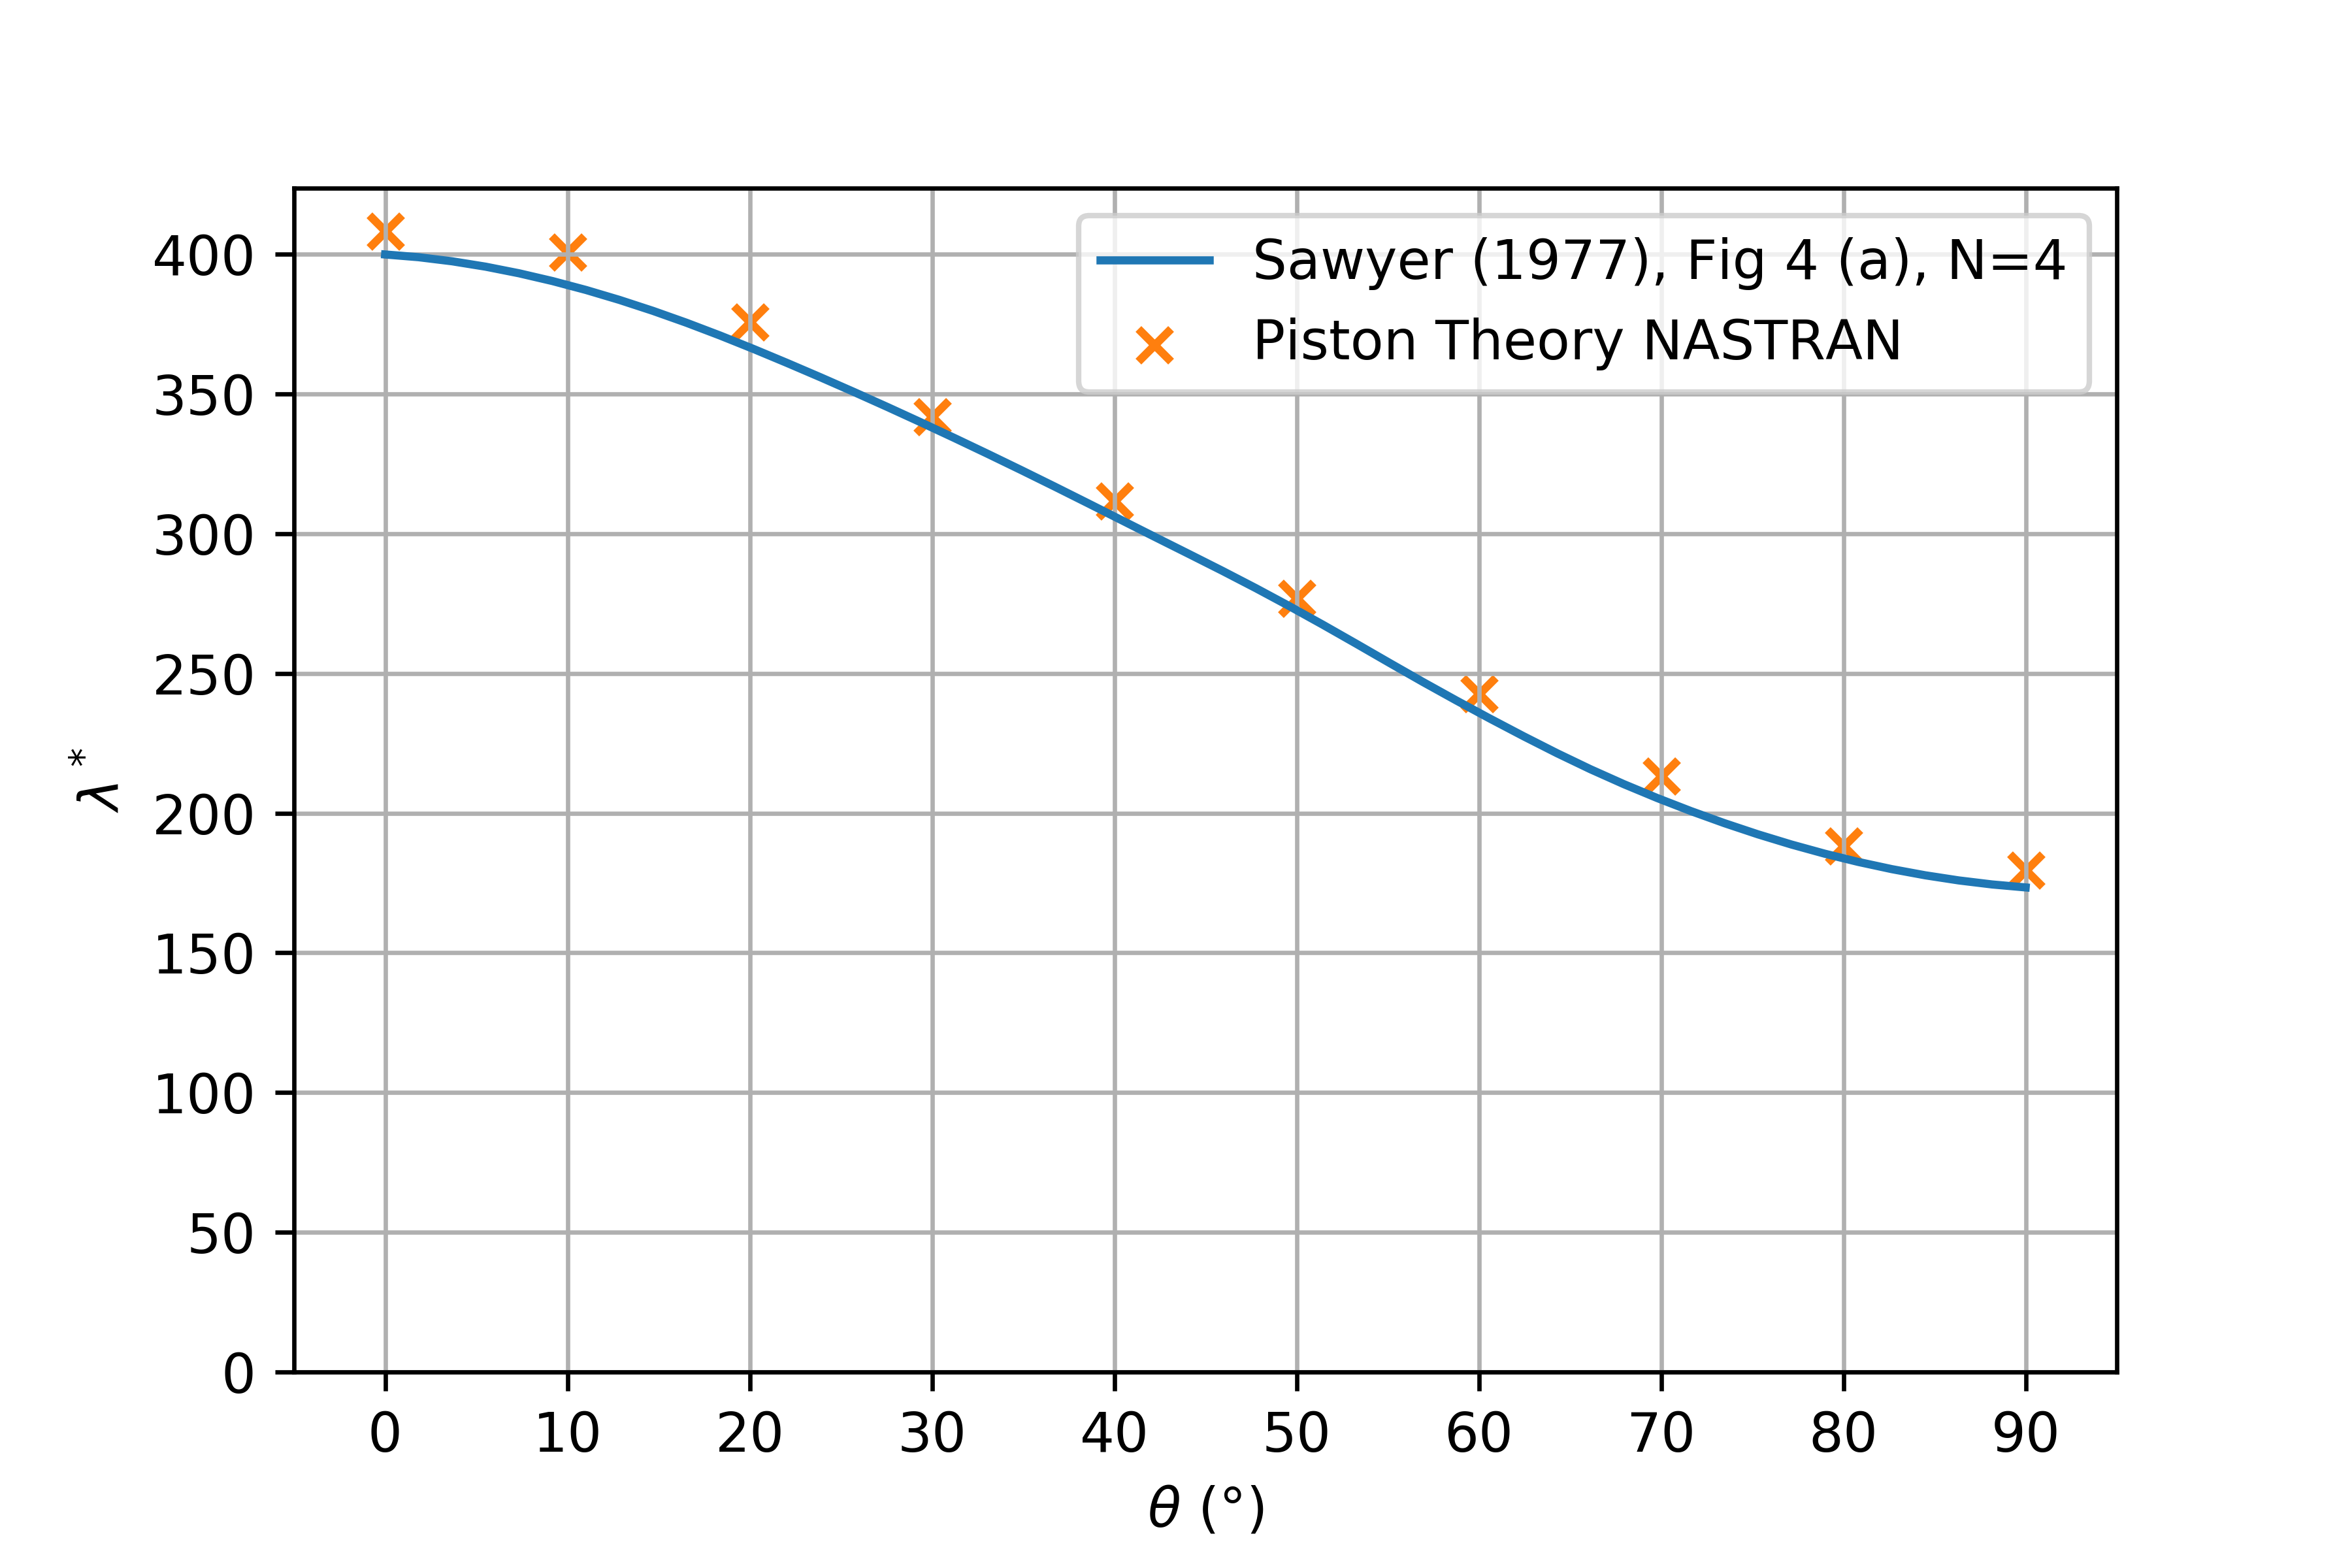
\includegraphics[width=0.7\linewidth]{figures/reference-77.png}
% \fonte{\cite{cook}.}
\label{fig-result-comp}
\end{figure}

% \subsection{Placa Quadrada com Reforçador Longitudinal}
